\documentclass[a4paper,11pt]{article}
% Various packages
\usepackage{siunitx}
\usepackage[utf8]{inputenc} % æøå
\usepackage[T1]{fontenc} % mere æøå
\usepackage[danish]{babel} % orddeling
\usepackage{verbatim} % så man kan skrive ren tekst
\usepackage{graphicx}
\graphicspath{{assets/}}
\usepackage{a4wide}
\usepackage{url}
\usepackage[left=2cm,top=2cm,bottom=1.5cm,right=2cm]{geometry}
\usepackage{amsmath}
\usepackage{amssymb}
\usepackage{amsthm}
\usepackage{wrapfig}
\usepackage{fixme}
\usepackage{color}
\usepackage[makeroom]{cancel}
\usepackage{pstricks}
\usepackage{pdfpages} % include pdf
\usepackage{forest}
\usepackage{float} % Use [H] in figures
\usepackage{subcaption} % For subfigures
\usepackage{color} % May be necessary if you want to color links
%\usepackage{xcolor} \pagecolor[rgb]{0,0,0} \color[rgb]{1,1,1}
\usepackage{nameref}
\usepackage{hyperref} % Make references clickable
\usepackage[nameinlink,capitalize]{cleveref} % Make eq:refs be in style (1)
\usepackage[linesnumbered, commentsnumbered, lined, ruled, vlined,
%noend  % Have no ⌊-like symbol to indicate end of scope in pseudocode
]{algorithm2e} % Doc: https://goo.gl/6bC1qZ

\crefname{equation}{}{Equations}

% Ændr på navnene der vises når man bruger \autoref{label}
\def\sectionautorefname{Sektion}
\renewcommand{\equationautorefname}{Ligning}
\def\figureautorefname{Figur}
\AtBeginDocument{\renewcommand{\ref}[1]{\autoref{#1}}}

% Sæt \ref{} til at kalde \autoref{}
\AtBeginDocument{\renewcommand{\ref}[1]{\autoref{#1}}}

% Ændr ''*'' i math-felter til \cdot
\DeclareMathSymbol{*}{\mathbin}{symbols}{"01}

% Sæt farver for interne referencer og links
\definecolor{darkblue}{RGB}{25,25,112}
\hypersetup{
	colorlinks=true,    %set true if you want colored links
	linktoc=all,        %set to all if you want both sections and subsections linked
	linkcolor=darkblue, %choose some color if you want links to stand out
	filecolor=blue,     %
	citecolor=black,    %
	urlcolor=cyan,      %
}

% Set indentation to 0:
\setlength\parindent{0pt}

% Keywords relateret til algorithm2e pakken
\newcommand{\True}{\textbf{true}}\newcommand{\False}{\textbf{false}}
\SetStartEndCondition{ }{}{}%
\SetKwProg{Fn}{def}{\string:}{}
\SetKw{KwTo}{to}
\SetKwFor{For}{for}{}{}%
\SetKwFor{ForEach}{foreach}{}{}%
\SetKwIF{If}{ElseIf}{Else}{if}{}{elif}{else}{end}%
\SetKwFor{While}{while}{}{end}\SetKwProg{Fn}{}{}{}
\SetKwInOut{Input}{input}\SetKwInOut{Output}{output}
\setlength{\algomargin}{3em}\DontPrintSemicolon

\newcommand{\longspace}{{\ \ \ \ \ \ \ \ \ \ \ \ \ \ }}
% \renewcommand{\P}{{\mathbb P}}
\newcommand{\R}{{\mathbb R}}
\newcommand{\E}{{\mathbb E}}
\newcommand{\event}{{\mathcal{E}}}
\newcommand{\parfrac}[1]{\frac{\partial}{\partial #1}}
\renewcommand{\num}{{\textrm{num} }}
\newcommand{\size}{{\textrm{size} }}
\newcommand{\ift}{{\textrm{if } }}

\newcommand{\pfrac}[2]{\left( \frac{#1}{#2} \right)}

% Dynamiske (), <>, ceil, floor
\newcommand{\p}[1]{\left( #1 \right)}
\newcommand{\pbig}[1]{\big( #1 \big)}
\newcommand{\pBig}[1]{\Big( #1 \Big)}
\newcommand{\pbigg}[1]{\bigg( #1 \bigg)}
\newcommand{\curly}[1]{\left\{ #1 \right\}}
\renewcommand{\square}[1]{\left[ #1 \right]}
\newcommand{\larr}[1]{\left< #1 \right>}
\newcommand{\ceil}[1]{\left\lceil #1 \right\rceil}
\newcommand{\floor}[1]{\left\lfloor #1 \right\rfloor}

\renewcommand{\P}[1]{\mathbb{P} \square{ #1 } }

\author{Søren Mulvad, rbn601}

\title{Eksamensdisposition - Kapitel 3}

\begin{document}
\maketitle

\begin{itemize}
  \item \textbf{Markovs ulighed}
  \item \textbf{Chebyshevs ulighed}
  \item \textbf{Two-point sampling}
  \begin{itemize}
    \item Algoritme 1
    \item Algoritme 2
    \item Sandsynlighed for algoritme 2 fejler
  \end{itemize}
  \item \textbf{The Coupon Collector's Problem}
  \begin{itemize}
    \item Forventet antal runder
    \item Sandsynlighed for flere end $r$ runder
  \end{itemize}
\end{itemize}


%%%%%%%%%%%%%%%%%%%%%%%%%%%%%%%%%%%%%%%%%%%%%%%%%%%%%%%%%%%
%%%%%%%%%%%%%%%%%%%%%%%%%%%%%%%%%%%%%%%%%%%%%%%%%%%%%%%%%%%
%%%%%%%%%%%%%%%%%%%%%%%%%%%%%%%%%%%%%%%%%%%%%%%%%%%%%%%%%%%
\newpage
%%%%%%%%%%%%%%%%%%%%%%%%%%%%%%%%%%%%%%%%%%%%%%%%%%%%%%%%%%%
%%%%%%%%%%%%%%%%%%%%%%%%%%%%%%%%%%%%%%%%%%%%%%%%%%%%%%%%%%%
%%%%%%%%%%%%%%%%%%%%%%%%%%%%%%%%%%%%%%%%%%%%%%%%%%%%%%%%%%%
\section{Eksamensdisposition - Kapitel 3}

\subsection{Markovs ulighed}
Givet en tilfældig variabel $X \geq 0$ og $t > 0$, så:
\begin{align}
  \P{X \geq t} \leq \frac{\E{X}}{t} \label{eq:markov}
\end{align}

Såfremt $\E{X} \neq 0$ og $k > 0$ kan vi omskrive det til:
$$
\mathbb{P} \Big[X \geq \underbrace{k * \E{X}}_{t} \Big] \leq \frac{1}{k}
$$

\textit{\textbf{Bevis:}}
\begin{align}
  \E{X}
  &= \sum_x x \P{X = x} \nonumber \\
  &\geq \sum_{x \geq t} x \P{X = x} \label{eq:summer-x-over-t} \\
  &\geq \sum_{x \geq t} t \P{X = x} \label{eq:summer-t-over-t} \\
  &= t \P{X \geq t} \label{eq:markov-res}
\end{align}

Hvor uligheden i \cref{eq:summer-x-over-t} gælder da vi antager $X \geq 0$ og vi summerer over potentielt færre led, uligheden i \cref{eq:summer-t-over-t} gælder da $t \leq x$ i vores summering, og \cref{eq:markov-res} gælder da vi blot indsætter $x \geq t$ fra vores summering i selve sandsynligheden.

\subsection{Chebyshevs ulighed}
Givet en tilfældig variabel $X$ med forventet værdi $\mu_X$, hvor $\sigma_X > 0$ og $t > 0$, så:
\begin{align}
  \P{|X - \mu_X| \geq t \sigma_X} \leq \frac{1}{t^2} \label{eq:chebyshev}
\end{align}

\textit{\textbf{Bevis:}}
\begin{align}
  \P{|X - \mu_X| \geq t \sigma_X}
  &= \P{(X - \mu_X)^2 \geq t^2 {\sigma_X}^2} \nonumber \\
  &\leq \frac{\E{(X - \mu_X)^2}}{t^2 {\sigma_X}^2} \label{eq:bruger-markov} \\
  &= \frac{{\sigma_X}^2}{t^2 {\sigma_X}^2} \label{eq:varians-def} \\
  &= \frac{1}{t^2} \nonumber
\end{align}

Her benytter vi Markovs ulighed i \cref{eq:bruger-markov} og selve definitionen på varians $\sigma^2$ i \cref{eq:varians-def}.

\begin{figure}[H]
  \begin{center}
  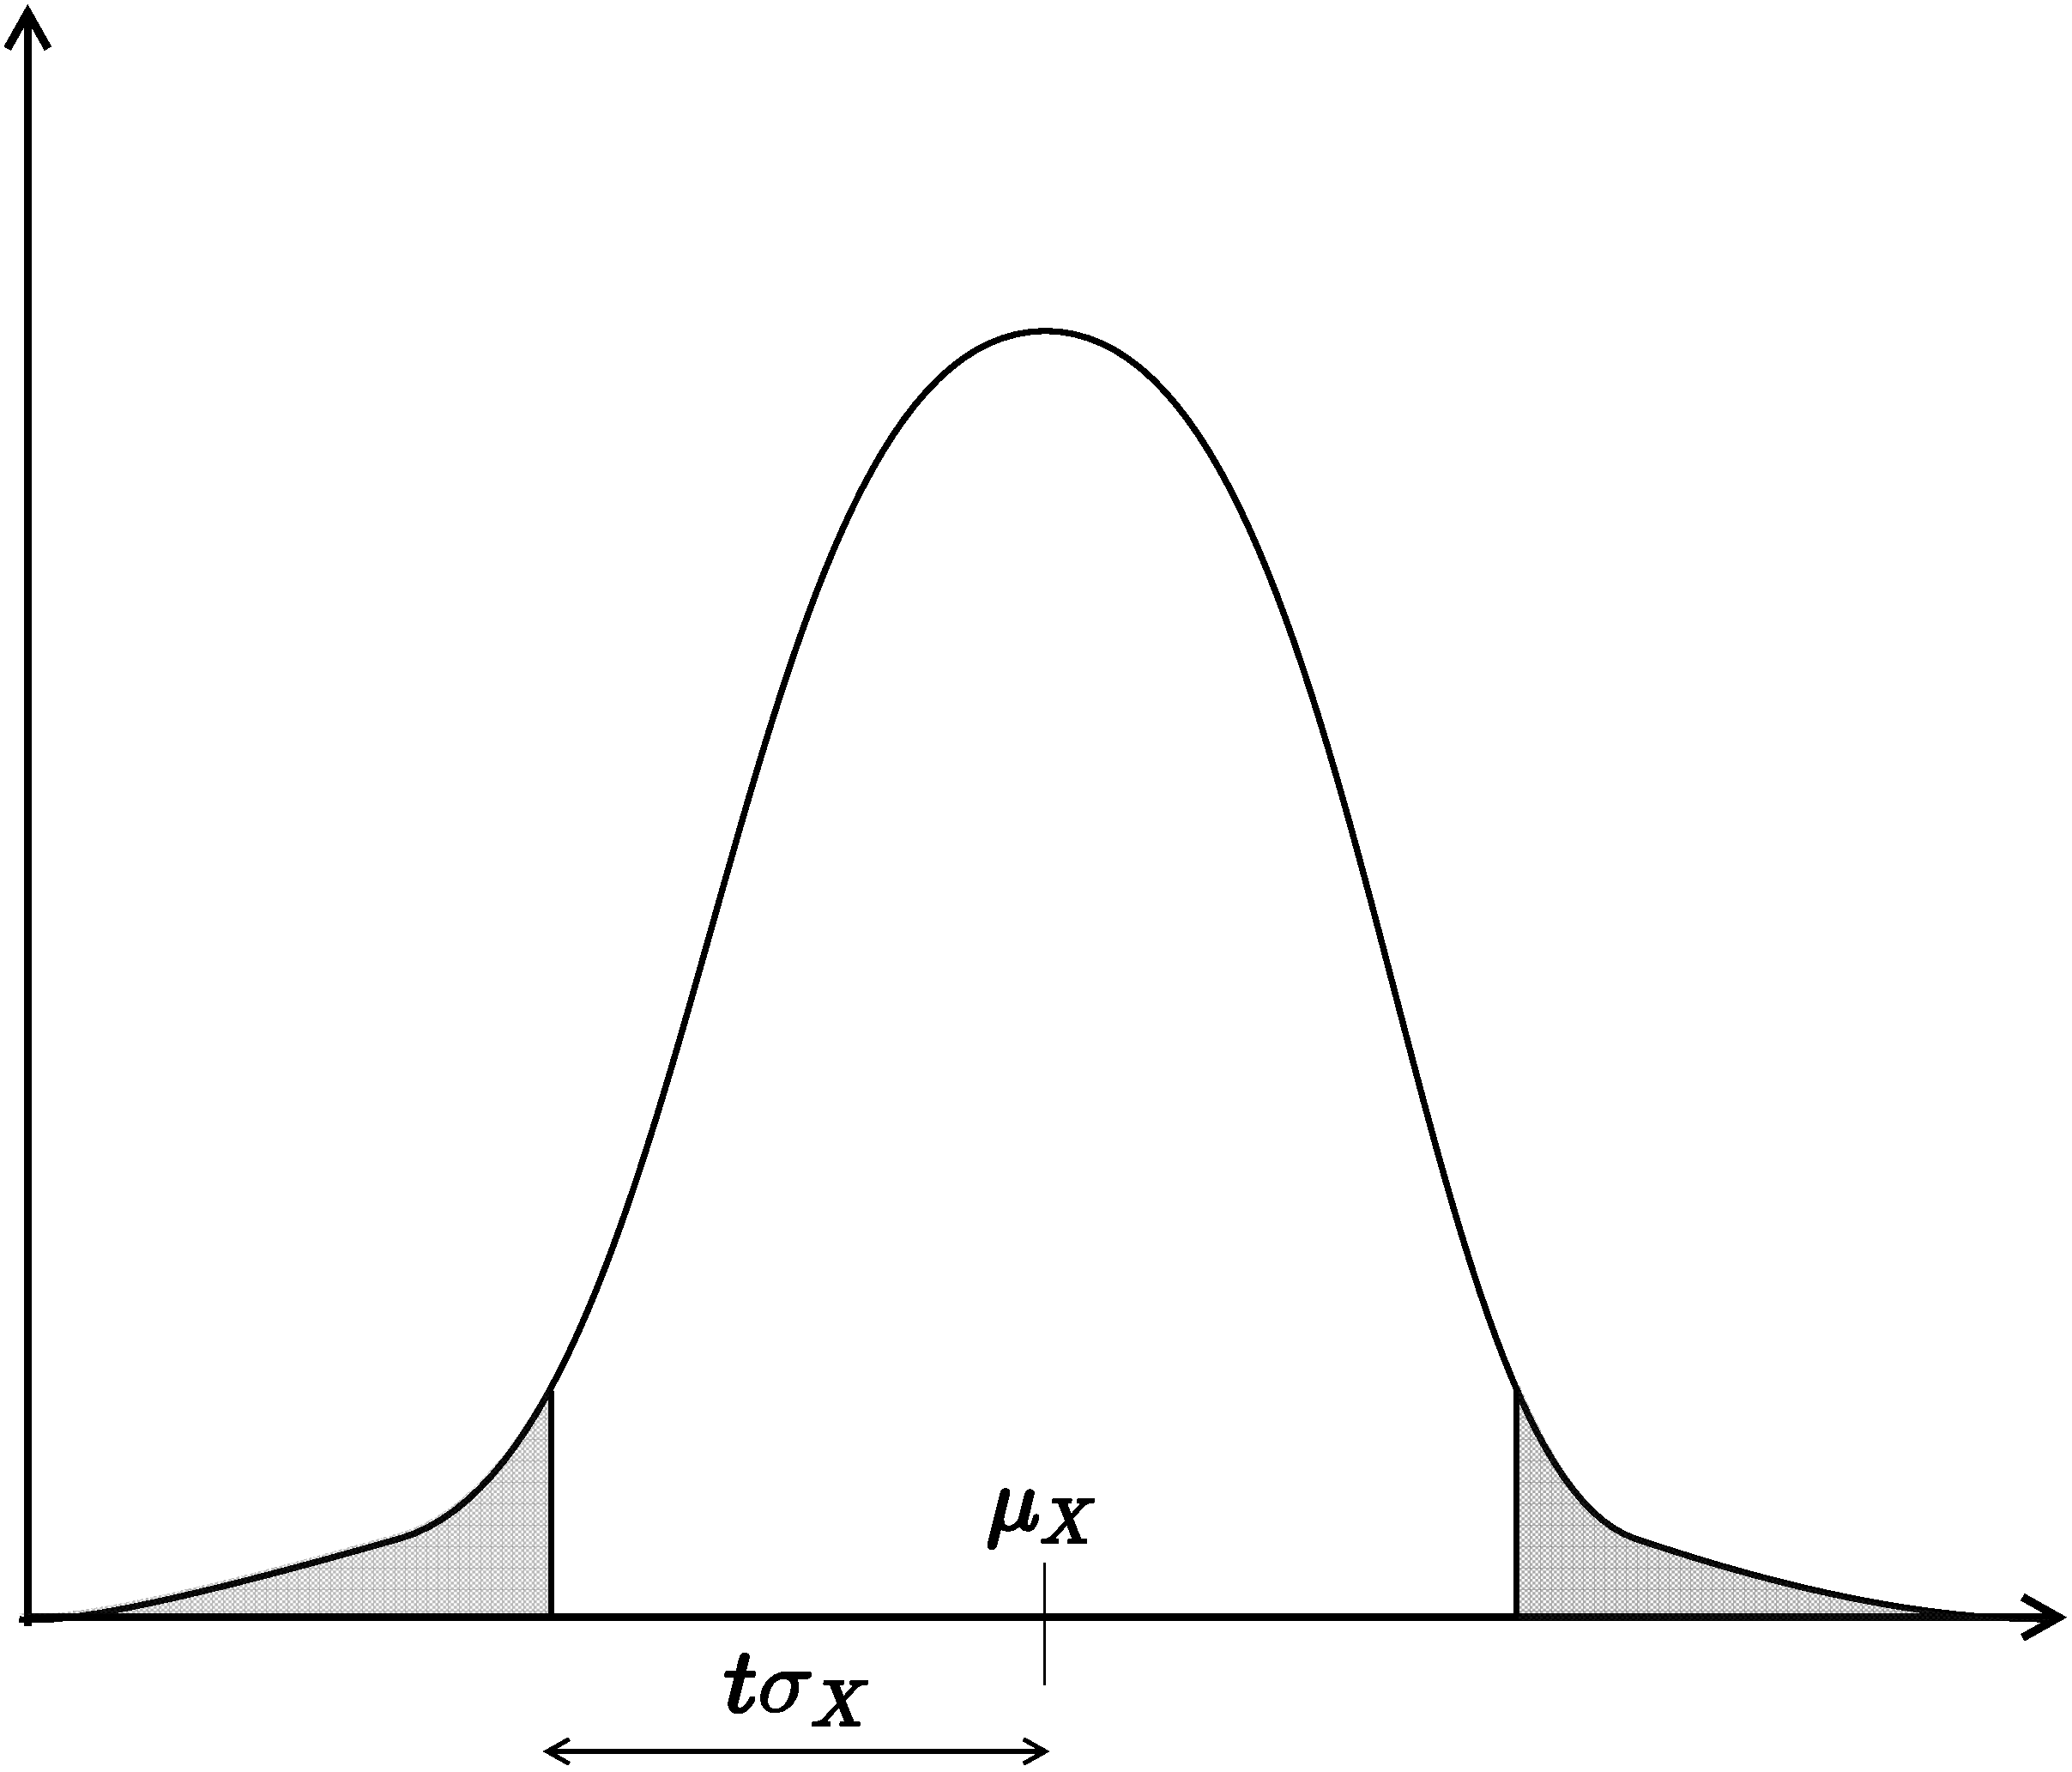
\includegraphics[width=0.4\textwidth]{chebyshev.pdf}
  \end{center}
  \caption{Illustration af Chebyshevs ulighed. Summen af de skraverede områder er $\leq 1/t^2$.}
  \label{fig:chebyshev}
\end{figure}










\section{Two-point Sampling}
Et decision-problem kan repræsenteres om en delmængde (et sprog) $L \subseteq \{0, 1\}^\ast = \{\emptyset, 0, 1, 00, 01, \dots \}$.

En korrekt algoritme $A^\ast$ for $L$ skal opfylde
\begin{align*}
  x \in L \rightarrow A^\ast(x) = 1\\
  x \notin L \rightarrow A^\ast(x) = 0
\end{align*}

\begin{figure}[H]
  \begin{center}
  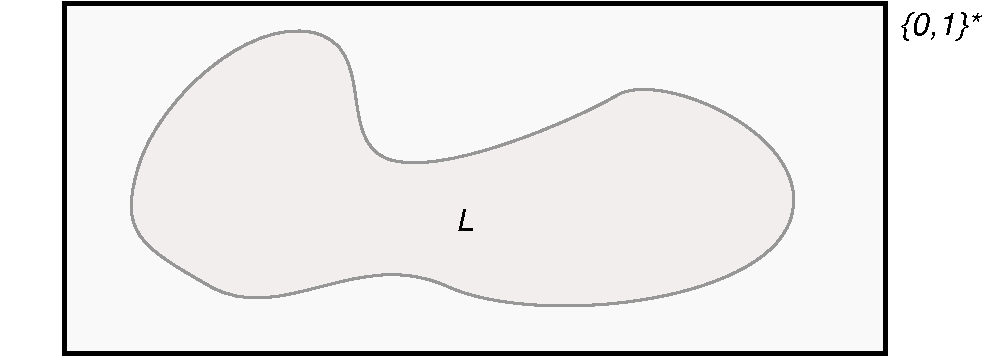
\includegraphics[width=0.7\textwidth]{sprog.pdf}
  \end{center}
  \caption{En delmængde (sprog) $L \subseteq \{0, 1\}^\ast$}
  \label{fig:sprog}
\end{figure}

Lad os nu betragte en Monte Carlo algoritme $A$ (one-sided error), så:
\begin{align*}
  x &\in L \rightarrow A(x) = 1 \text{ med sandsynlighed $\geq 1/2$}\\
  x &\notin L \rightarrow A(x) = 0 \text{ med sandsynlighed $1$}
\end{align*}

Antag at algoritme $A$ bruger $\lg n$ tilfældige bits repræsenteret som et tal $r \in \{0, ..., n-1 \}$ hvor $n$ er et primtal. I følgende bruger vi notationen $A(x, r)$ for at beskrive outputtet af $A$ på input $x$, hvor $A$ vælger den tilfældige bitstreng $r$. Og lad os i fejlsandsynlighederne antage, at vores konkrete $x \in L$ så det korrekte svar er 1.\\

\textbf{Algoritme 1 - $t \lg n$ random bits}\\
Vælg $t$ tal $r_0, \dots, r_{t-1} \in \{0, \dots, n-1\}$ uafhængigt og uniformt tilfældigt.\\
Beregn $A(x, r_0), \dots, A(x, r_{t-1})$. Hvis vi en enkelt gang ser tallet 1 er det bevis på $x \in L$, ellers hvis vi \emph{alle} gange får 0 vælger vi det som output.\\

Så vil fejlsandsynligheden være $< \pfrac{1}{2}^t = 1/2^t$.\\

Problemet ved denne tilgang er, at vi skal vælge $t \lg n$ random bits. Hvis vi f.eks. vælger $t = 2$ skal vi bruge $2 \ln n$ random bits for en fejlsandsynlighed $< 1/4$.\\

\textbf{Algoritme 2 - $2 \lg n$ random bits}\\
Vælg $a, b \in \curly{0, \dots, n-1}$ uafhængigt og uniformt tilfældigt.\\

Da vi antager $n$ er et primtal, så kan man vise at, for $X_i = (a * i + b) \bmod n$ vil $X_i$ og $X_j$ hvor $i \neq j$ være uniformt distribueret i $0, \dots, n-1$ og parvist uafhængige (kan blot antages, skal ikke bevises).\\

Med den info, lad $r_i = (a * i + b) \mod n$ for $i = 0, \dots, t-1$.\\
Igen beregner vi $A(x, r_0), \dots, A(x, r_{t-1})$ og vælger 1 såfremt den optræder bare én gang, ellers 0.\\

Nu bruger vi kun $2 \lg n$ random bits.

\subsection{Sandsynlighed for at algoritme 2 fejler}
Vi skal ligesom i randomized selection bruge, at givet parvis uafhængige stokastiske variable $Y_1, \dots, Y_m$ hvor vi lader $Y = \sum_{i=1}^m Y_i$, da er
\begin{align}
  {\sigma_Y}^2 = \sum_{i=1}^m {\sigma_{Y_i}}^2 \label{eq:parvis-uaf}
\end{align}\vspace{2em}

For $i = 0, \dots, t-1$ lader vi $Y_i = A(x, r_i)$. Lad nu $Y = \sum_{i=1}^{t-1} Y_i$.

Da kan vi beregne den forventede værdi:
\begin{align}
  \mu_Y = \sum_{i=0}^{t-1} \mu_{Y_i} = \sum_{i=0}^{t-1} p = tp \geq \frac{t}{2} \label{eq:mu-y-ulighed}
\end{align}
Idet vi lader symbolet $p = \P{Y_i = 1} \geq \frac{1}{2}$.\\

Derudover har vi jf. \cref{eq:parvis-uaf}:
\begin{align}
  {\sigma_Y}^2
  &= \sum_{i=0}^{t-1} {\sigma_{Y_i}}^2
  = \sum_{i=0}^{t-1} p(1-p)
  \leq \frac{t}{4} \label{eq:bern} \\
  &\Updownarrow \nonumber  \\
  \sigma_Y &= \frac{\sqrt{t}}{2}  \label{eq:std-dev}
\end{align}

I \cref{eq:bern} bruger vi at de stokastiske variable $Y_i$ er Bernoulli trials som har variansen $\sigma_{Y_i}^2 = p*(1-p)$ hvor $p = \P{Y_i = 1}$ og at udtrykket $p(1 - p)$ er størst når $p = 1/2$ og da bliver $1/4$.\\
I \cref{eq:std-dev} tager vi kvadratroden og får herved standardafvigelsen.


Da kan vi beregne sandsynligheden for at algoritme 2 fejler til:
\begin{align}
  \P{\text{Algoritme 2 fejler}} &= \P{Y = 0} \label{eq:p-y-lig-0} \\
  &\leq \P{| Y - \mu_Y| \geq \frac{t}{2}} \label{eq:traak-middelvaardi} \\
  &= \P{|Y - \mu_Y| \geq \sqrt{t} \frac{\sqrt{t}}{2}} \nonumber \\
  &\leq \frac{1}{(\sqrt{t})^2} \label{eq:benyt-cheby}\\
  &\leq \frac{1}{t} \nonumber
\end{align}

I \cref{eq:p-y-lig-0} bruger vi, at algoritmen fejler (givet vores antagelse at svaret \emph{er} 1) når vi får 0 i alle vores trials.\\
I \cref{eq:traak-middelvaardi} indsætter vi ulighed \cref{eq:mu-y-ulighed} for $\mu_Y$. Grunden til vi får '$\leq$'-tegnet i denne ligning er pga. vi tager den absolutte værdi, hvorved der kommer ''to muligheder'' for at det udtryk kan være større end brøken, hvilket der ikke gjorde i \cref{eq:mu-y-ulighed}.\\
I \cref{eq:benyt-cheby} benytter vi Chebyshev's ulighed.\\

Hermed har vi altså bestemt, at vi kan få en relativt lav sandsynlighed for fejl selvom vi kun bruger $2 \lg n$ random bits.







\newpage
\section{The Coupon Collector's Problem}
Betragt følgende eksperiment. Vi har $n$ unikke unikke kupontyper:
\begin{figure}[H]
  \begin{center}
  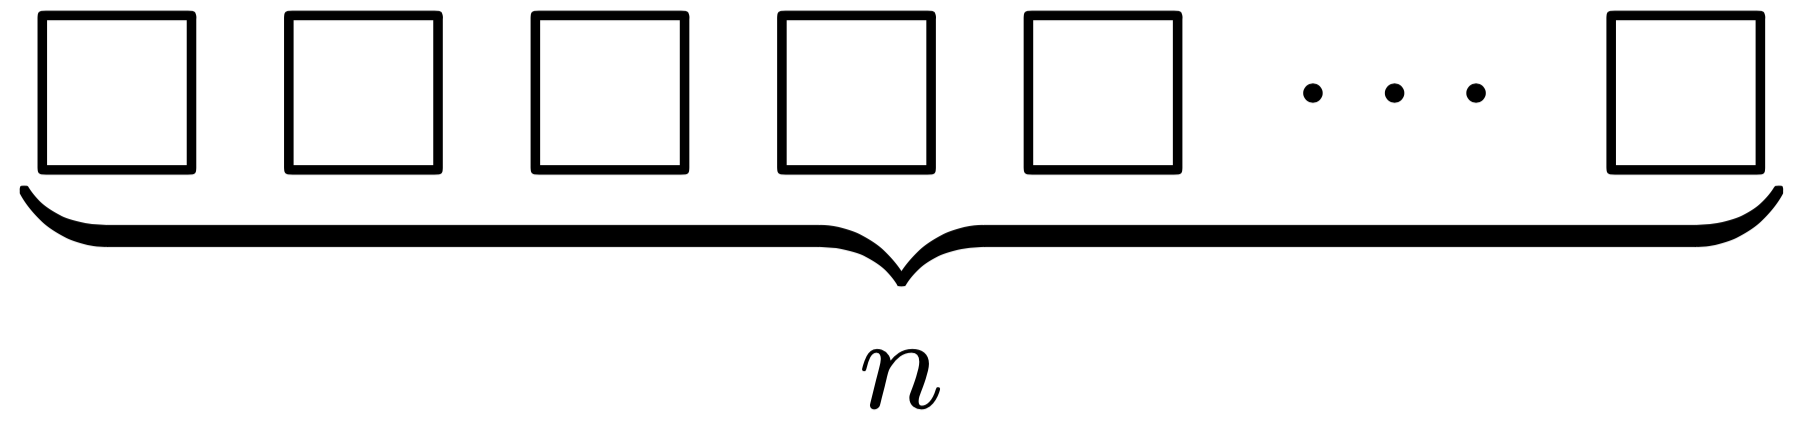
\includegraphics[width=0.3\textwidth]{coupon.png}
  \end{center}
  %\caption{}
  \label{fig:coupon}
\end{figure}

I hver runde vælges en kupon-type uafhængigt og uniformt tilfældigt. Vi stopper når alle kupon-typer er valgt. Hvor mange runder vil der være i dette eksperiment?\\

For at besvare dette skal vi først definere hvad en epoke er. For $i = 0, \dots, n-1$ består den $i$'te epoke af de runder, der starter lige efter den $i$'te succes og slutter i runden med $(i+1)$'te succes, hvor en succes er defineret som at vælge en kupontype vi ikke har set før. Eksempelvis kunne vi have:
$$
  \underbrace{C_2,}_{\text{Epoke 0}} \underbrace{C_2, C_1}_{\text{Epoke 1}}, \underbrace{C_2, C_2, C_3}_{\text{Epoke 2}}, \dots
$$


\subsection{Forventet antal runder}
For $i = 0, \dots, n-1$ lader vi $Y_i$ være længden af epoke $i$. Lad nu $Y = \sum_{i=0}^{n-1} Y_{i}$. Vi har, at sandsynligheden i den $i$'te epoke for at finde en ny kupon er antallet af ufundne kuponer $n-i$ over alle de forskellige kupontyper $n$:
$$
  p_i = \frac{n-i}{n}
$$

Bruger vi, at dette er geometrisk distribueret får vi:
$$
  \mu_{Y_i} = \frac{1}{p_i} = \frac{n}{n-i}
$$

Da kan vi beregne:
\begin{align*}
  \mu_Y
  = \sum_{i=0}^{n-1} \mu_{Y_i}
  = \sum_{i=0}^{n-1} \frac{n}{n-i}
  = n \sum_{i=1}^n \frac{1}{i}
  = n H_n
  = n \ln n + \Theta(n)
  = O(n \ln n)
\end{align*}


\subsection{Sandsynlighed for flere end $r$ runder}
For $i = 1, \dots, n$ og $r \in \mathbb{N}_0$ defineres følgende begivenhed:\\
$\event_i^r$: Kupontype $i$ vælges \emph{ikke} i de første $r$ runder.\\

Da er begivenheden at mindst én kupontype ikke vælges i de $r$ første runder $\bigcup_{i=1}^n \event_i^r$. Denne sandsynlighed er naturligvis ækvivalent med sandsynligheden for, at der totalt set vil være flere end $r$ runder før vi er færdig. Da kan vi bestemme sandsynligheden for flere end $r$ runder til:
\begin{align}
  \P{\bigcup_{i=1}^n \event_i^r}
  &\leq \sum_{i=1}^n \P{\event_i^r} \label{eq:bruger-union-bound} \\
  &= \sum_{i=1}^n \pfrac{n-1}{n}^r \label{eq:sandsynlighed} \\
  &= \sum_{i=1}^n \p{1 - \frac{1}{n}}^r \nonumber \\
  &\leq \sum_{i=1}^n \p{e^{-1/n}}^r \label{eq:1plusx}\\
  &= n e^{-r/n} \nonumber
\end{align}

Hvor vi i \cref{eq:bruger-union-bound} bruger Union Bound, i \cref{eq:sandsynlighed} har at $\P{\event_i^1} = \frac{n-1}{n}$ hvor det skal ske $r$ gange og i \cref{eq:1plusx} bruger regnereglen $1 + x \leq e^x$ for alle $x \in \R$.


\subsubsection{Eksempel på beregning}
Lad os vælge $r = \beta n \ln n$. Da vil
$$
  \P{\text{Mere end $r$ runder}} \leq n * e^{- \beta \ln n} = n * n^{- \beta} = n^{1 - \beta}
$$
For $\beta = 2$ får vi:
$$
  \P{\text{Mere end $2 n \ln n$ runder}} \leq \frac{1}{n}
$$

Altså er sandsynligheden for at laver flere end dobbelt så mange runder som forventet relativt lille.



\end{document}
